\documentclass[10pt]{article}
\usepackage[a4paper, total={6in,9in}]{geometry}
\usepackage[parfill]{parskip}    	
\usepackage{graphicx,caption,fancyhdr,xcolor,pdfpages,setspace}
\usepackage{minted}
\usepackage{xcolor}
\usepackage[
        colorlinks = true,
        allcolors  = darkgray
]{hyperref}



\newcommand{\wrt}[1]{\mathrm{d}#1}


\setlength{\fboxsep}{0.5em}



\urlstyle{same}
\renewcommand{\footnoterule} % Push footnotes to the bottom of the pagehttps://www.overleaf.com/project/634eca5f6262ed6dd715c645
	{\vfill\kern -3pt \hrule width 0.4\columnwidth \kern 2.6pt}

\makeatletter
\title{Digital Design with HDL Lab 2}
\let\Title\@title
\author{Y3862181 \& Y3899129}
\let\Author\@author
\date{Autumn Term, 2022}
\let\Date\@date
\makeatother


\fancypagestyle{content}{
    \renewcommand{\headrulewidth}{0.4pt}
    \renewcommand{\footrulewidth}{0.4pt}
    \setlength{\headheight}{15pt}
    
	\fancyhf{}
	\fancyhead[L]{\Author}
	\fancyhead[R]{\Title}
	\fancyfoot[L]{\Date}
	\fancyfoot[R]{\thepage}
}
\onehalfspacing
\begin{document}
\begin{titlepage}
\centering
{\Huge Lab Report 2}

\vspace{3cm}

{\LARGE \textbf{ Digital Design with HDL}}

\vspace{3cm}

{\huge Y3862181 \& Y3899129}

\vspace{2cm}


{\large Autumn Term, 2022}
\vfill

{\itshape University of York}
\end{titlepage}

\tableofcontents
\newpage

\pagestyle{content}
\section{Introduction}
This lab focuses on understanding and implementing schematics involving sequential logic.

Part A exposes the implementation of four different D-type registers (synchronous reset without enable, asynchronous reset without enable, synchronous reset with enable and asynchronous reset with enable).

Part B focuses on real applications involving counters, debouncers and decoders. The schematic to be implemented is a 7-segment display controller that gets reset and enable as inputs. Both of those inputs run through a debounce circuit in case of push-button oscillations. The reset input resets an internal counter that counts from 0 to 99 in BCD (Binary Coded Decimal) and every time there is a steady signal at the enable input the counter increments (or overflows in the case of 99). The counter outputs two 4-bit BCD lines (one for the ones and one for the tens). These outputs are then decoded with BCD to 7-segment decoders. 




\newpage

\section{Task A: Implementation of Sequential Elements}
\subsection{VHDL Code \texttt{(sequential\_logic.vhd)}}
\begin{minted}{vhdl}
library IEEE;
use IEEE.STD_LOGIC_1164.ALL;
use IEEE.NUMERIC_STD.ALL;
-- Implementation of four variations of D-type registers:
-- 1) Synchronous reset without enable
-- 2) Asynchronous reset without enable
-- 3) Synchronous reset with enable
-- 4) Asynchronous reset with enable
entity sequential_logic is
    Port ( -- Clock input (common for all registers)
           clk   : in STD_LOGIC; 
           -- Enable signal (common for all registers)
           en    : in STD_LOGIC;
           -- Reset signal (common for all registers)
           rst   : in STD_LOGIC; 
           -- Data input (common for all registers)
           input : in STD_LOGIC_VECTOR (3 downto 0); 
           -- output of register (1)
           output_sync_rst       : out STD_LOGIC_VECTOR (3 downto 0); 
           -- output of register (2)
           output_async_rst      : out STD_LOGIC_VECTOR (3 downto 0); 
           -- output of register (3)
           output_sync_rst_enbl  : out STD_LOGIC_VECTOR (3 downto 0); 
           -- output of register (4)
           output_async_rst_enbl : out STD_LOGIC_VECTOR (3 downto 0)); 
end sequential_logic;
architecture Behavioral of sequential_logic is
begin

-- D-type register with synchronous reset without enable (1) 
d_reg_sync_rst: process (clk)
begin
    if (rising_edge(clk)) then
        if (rst = '1') then
            output_sync_rst <= (others => '0');
        else
            output_sync_rst <= input;
        end if;
    end if;
end process d_reg_sync_rst;
-- D-type register with asynchronous reset without enable (2)
d_reg_async_rst: process (clk, rst)
begin
    if (rst = '1') then
        output_async_rst <= (others => '0');
    elsif (rising_edge(clk)) then
        output_async_rst <= input;
    end if;
end process d_reg_async_rst;

-- D-type register with synchronous reset with enable (3)
d_reg_sync_rst_enbl: process (clk)
begin
    if (rising_edge(clk)) then
        if (rst = '1') then
            output_sync_rst_enbl <= (others => '0');
        elsif (en = '1') then
            output_sync_rst_enbl <= input;
        end if;
    end if;
end process d_reg_sync_rst_enbl;

-- D-type register with asynchronous reset with enable (4)
d_reg_async_rst_enbl: process (clk, rst)
begin
    if (rst = '1') then
        output_async_rst_enbl <= (others => '0');
    elsif ( (rising_edge(clk)) and (en = '1') ) then
        output_async_rst_enbl <= input;
    end if;
end process d_reg_async_rst_enbl;

end Behavioral;

\end{minted}
\newpage

\subsection{VHDL Testbench \texttt{(sequential\_logic\_tb.vhd)}}
\begin{minted}{vhdl}
library IEEE;
use IEEE.STD_LOGIC_1164.ALL;

-- A testbench to confirm the correct operation of the sequential components

entity sequential_logic_tb is
end sequential_logic_tb;

architecture Behavioral of sequential_logic_tb is

constant clk_period : time := 10 ns;
    
signal clk                   : STD_LOGIC;
signal en                    : STD_LOGIC;
signal rst                   : STD_LOGIC;
signal input                 : STD_LOGIC_VECTOR (3 downto 0);
signal output_sync_rst       : STD_LOGIC_VECTOR (3 downto 0);
signal output_async_rst      : STD_LOGIC_VECTOR (3 downto 0);
signal output_sync_rst_enbl  : STD_LOGIC_VECTOR (3 downto 0);
signal output_async_rst_enbl : STD_LOGIC_VECTOR (3 downto 0);

begin

-- Clock process
clk_process :process
begin
    clk <= '0';
    wait for clk_period/2;
    clk <= '1';
    wait for clk_period/2;
end process;

UUT : entity work.sequential_logic
    PORT MAP (
        clk => clk,
        en => en,
        rst => rst,
        input => input,
        output_sync_rst => output_sync_rst,
        output_async_rst => output_async_rst,
        output_sync_rst_enbl => output_sync_rst_enbl,
        output_async_rst_enbl => output_async_rst_enbl);
-- Testing strategy: First initial values are set (NOTE: input is set to a 
-- non-zero value in order to confirm the reset is working correctly). Then the
-- reset procedure is tested. After that, a new input value is set to test the 
-- registers without enable. Finally the enable is set to logic high in order to 
-- test the registers with enable

TEST : process
begin

    wait for 100 ns;
    wait until falling_edge(clk);
    
    -- Set initial values
    en <= '0';
    rst <= '0';
    input <= x"b";
    wait for clk_period;
    
    -- Reset the registers
    rst <= '1';
    wait for clk_period;
    rst <= '0';
    wait for clk_period;
    
    -- the registers with no enable should change on the rising edge
    input <= x"a";
    wait for clk_period;
    
    -- the registers with enable should change on the rising edge
    en <= '1';
    wait for clk_period;
    en <= '0';
    wait for clk_period;
    
    -- Reset the registers
    rst <= '1';
    wait for clk_period;
    rst <= '0';
    wait for clk_period; 
    
    wait;
end process;
end Behavioral;
\end{minted}
\subsection{Simulation}

It can be seen from the timing diagram in \autoref{fig:Simulation of Sequential Elements} that when the input value changes to `b', on the next rising clock edge, both of the no-enable registers change as expected. Then when the reset occurs, the asynchronous reset registers change instantly to `0' while the synchronous ones wait for a rising clock edge. The same behaviour applies to the second reset.


After the reset signal terminates, the two no-enable registers track the input (`b'). Then, when the input is changed (`a'), they track the input after the rising clock edge as expected while the registers with the enable require both an enable signal and a rising clock edge to change. 

\begin{figure}[ht]
    \centering
    \fbox{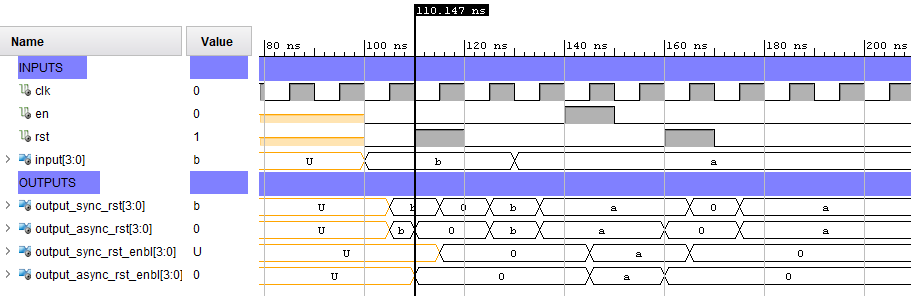
\includegraphics[width=0.9 \textwidth]{lab_2_A_simulation.png}}
    \caption{Simulation of sequential elements}
    \label{fig:Simulation of Sequential Elements}
\end{figure}
\newpage



\subsection{RTL Statistics}

In this section of the lab, four 4-bit registers were implemented and displayed as expected in both the RTL component statistics and the RTL hierarchical component statistics. 

\begin{minted}{text}

---------------------------------------------------------------------------------
Start RTL Component Statistics 
---------------------------------------------------------------------------------
Detailed RTL Component Info : 
+---Registers : 
	                4 Bit    Registers := 4     
---------------------------------------------------------------------------------
Finished RTL Component Statistics 
---------------------------------------------------------------------------------
---------------------------------------------------------------------------------
Start RTL Hierarchical Component Statistics 
---------------------------------------------------------------------------------
Hierarchical RTL Component report 
Module sequential_logic 
Detailed RTL Component Info : 
+---Registers : 
	                4 Bit    Registers := 4     
---------------------------------------------------------------------------------
Finished RTL Hierarchical Component Statistics
---------------------------------------------------------------------------------
\end{minted}


\newpage

\subsection{Schematic}
In contrast to the VHDL code for the sequential elements, it can be seen from the schematic in \autoref{fig:Schematic of Sequential Elements} that for the two asynchronous reset registers, the reset line is labelled as ``CLR" (CLEAR) instead of ``RST" (RESET). 

\begin{figure}[ht]
    \centering
    \fbox{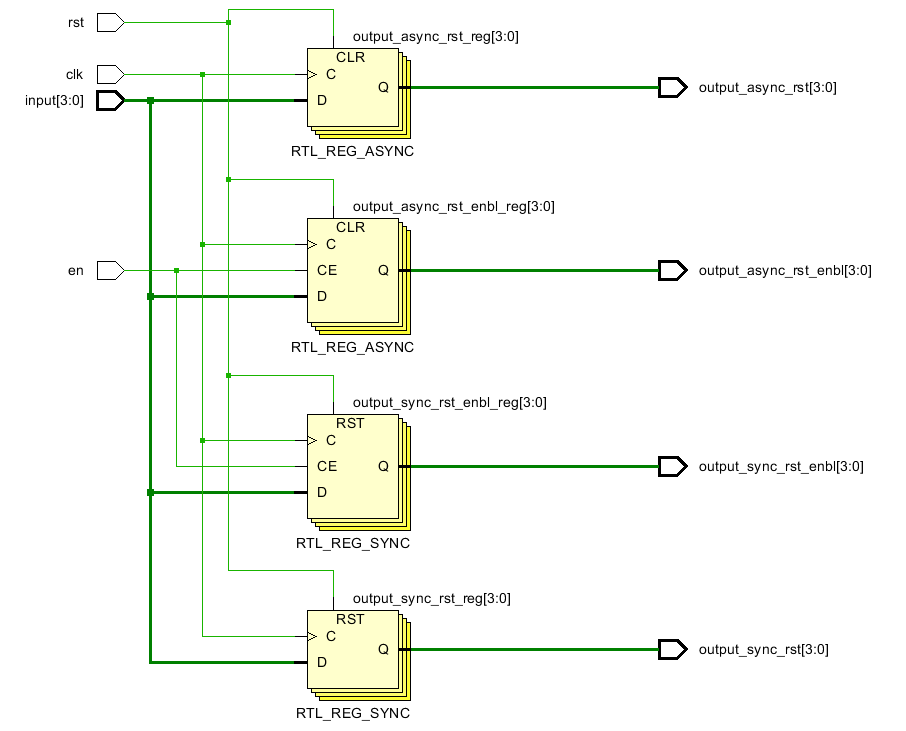
\includegraphics[width=0.97 \textwidth]{schematic.png}}
    \caption{Schematic of sequential elements}
    \label{fig:Schematic of Sequential Elements}
\end{figure}
\newpage


\section{Task B: Design of a 7-Segment Display Controller}
\subsection{Controller Implementation \texttt{(controller.vhd)}}
\begin{minted}{vhdl}
library IEEE;
use IEEE.STD_LOGIC_1164.ALL;
use IEEE.NUMERIC_STD.ALL;

-- Implementation of 7-segment display controller, which increments the shown 
-- number with every push of the enable button. Also clears the value with the 
-- use of a reset button

entity controller is
    Port ( -- Reset button input (un-debounced signal)
           rst_button   : in STD_LOGIC; 
           -- Enable button input (un-debounced signal)
           en_button    : in STD_LOGIC; 
           -- Clock input
           clk          : in STD_LOGIC; 
           -- Output to the ones 7-segment display
           display_ones : out STD_LOGIC_VECTOR (6 downto 0);  
           -- Output to the tens 7-segment display
           display_tens : out STD_LOGIC_VECTOR (6 downto 0)); 
end controller;


architecture Behavioral of controller is

-- Internal connections between the building blocks of the controller

signal deb_rst_button: STD_LOGIC; -- Filtered signal from the reset button
signal deb_en_button : STD_LOGIC; -- Filtered signal from the enable button
signal out_ones : UNSIGNED (3 downto 0); -- BCD internal bus for the ones counter
signal out_tens : UNSIGNED (3 downto 0); -- BCD internal bus for the tens counter

begin
-- Block to filter the signal from the reset button and implement an edge 
-- detection
DEBOUNCE_RST: entity work.DEBOUNCE
PORT MAP (
    clk => clk,
    sig => rst_button,
    deb_sig => deb_rst_button
);
-- Block to filter the signal from the enable button and implement an 
-- edge detection

DEBOUNCE_EN: entity work.DEBOUNCE
PORT MAP (
    clk => clk,
    sig => en_button,
    deb_sig => deb_en_button
);

-- Block to count in BCD from 0-99 using the filtered signals for the 
-- enable and the reset

COUNTER: entity work.COUNT
port map (
    clk => clk,
    rst => deb_rst_button,
    en => deb_en_button,
    out_ones => out_ones,
    out_tens => out_tens
);

-- 7-segment decoder for the ones display

DECODE_ONES: entity work.DECODER
port map(
    bcd_in => out_ones,
    seven_seg_out => display_ones
);

-- 7-segment decoder for the tens display

DECODE_TENS: entity work.DECODER
port map(
    bcd_in => out_tens,
    seven_seg_out => display_tens
);

end Behavioral;
\end{minted}
\newpage


\subsection{0-99 BCD Counter Implementation \texttt{(COUNT.vhd)}}
\begin{minted}{vhdl}
library IEEE;
use IEEE.STD_LOGIC_1164.ALL;
use IEEE.NUMERIC_STD.all;

-- Implementation of 0-99 counter using the single BCD counter component
-- The output of the counter consists of two separate BCD lines (ones and tens)
-- It features synchronous reset and enable signals

entity COUNT is
    Port ( clk      : in STD_LOGIC;               -- Clock signal 
           rst      : in STD_LOGIC;               -- Reset signal
           en       : in STD_LOGIC;               -- Count enable signal
           out_tens : out UNSIGNED (3 downto 0);  -- BCD output for the tens
           out_ones : out UNSIGNED (3 downto 0)); -- BCD output for the ones
end COUNT;

architecture Behavioral of COUNT is

-- Internal bus for the out_ones counter. It is used in order to access the bits 
-- of the out_ones in order to increment the out_tens
signal internal_ones : UNSIGNED (3 downto 0);

-- Internal signal to enable the counting of the tens counter
signal en_tens : STD_LOGIC;

begin

   -- Entity for the ones counter. The output of the counter is stored in the 
   -- internal_ones bus
   
   count_ones : entity work.bcd_counter
   port map (
        clk => clk,
        rst => rst,
        en => en,
        count_out => internal_ones
   );
   
   out_ones <= internal_ones;
   
   
   
   -- The count of the tens is enabled when the combination of the out_ones is 9 
   -- and the external enable is present
   
   en_tens <= '1' when (internal_ones = 9 and en = '1') else '0';
   
   -- Entity for the tens counter
   
   count_tens : entity work.bcd_counter
   port map (
        clk => clk,
        rst => rst,
        en => en_tens,
        count_out => out_tens
   );
   
end Behavioral;
\end{minted}
\newpage

\subsection{Single BCD Counter Implementation \texttt{(bcd\_counter.vhd)}}
\begin{minted}{vhdl}
library IEEE;
use IEEE.STD_LOGIC_1164.ALL;
use IEEE.NUMERIC_STD.all;

-- Implementation of a single BCD counter (counts from 0 to 9)
-- It features a synchronous reset and an enable signal
-- The output signal is of type UNSIGNED

entity bcd_counter is
    Port ( clk       : in STD_LOGIC; -- Clock signal
           en        : in STD_LOGIC; -- Counter enable signal
           rst       : in STD_LOGIC; -- Counter reset signal
           count_out : out UNSIGNED (3 downto 0)); -- The counter output (0 to 9)
end bcd_counter;

architecture Behavioral of bcd_counter is

-- Internal counter bus.
signal count_internal : UNSIGNED (3 downto 0);

begin

-- On the rising edge of the clock the BCD counter increments up to 9 whenever it 
-- is enabled and is cleared when the reset is set to logic high
bcd_counter: process ( clk )
begin
    if ( rising_edge ( clk ) ) then
        if ( rst = '1' ) then
            count_internal <= ( others => '0' );
        elsif ( en = '1' ) then 
            if ( count_internal = 9 ) then
                count_internal <= ( others => '0' );
            else
                count_internal <= ( count_internal + 1 );
            end if;
        end if;
    end if;  
end process bcd_counter;

-- Setting the output of the counter to the value of the internal bus
count_out <= count_internal;
end Behavioral;
\end{minted}
\newpage



\subsection{Decoder Implementation \texttt{(DECODER.vhd)}}
\begin{minted}{vhdl}
library IEEE;
use IEEE.STD_LOGIC_1164.ALL;
use IEEE.NUMERIC_STD.all;

-- Implementation of a BCD to 7-segment display decoder

entity DECODER is
    Port ( bcd_in        : in  UNSIGNED (3 downto 0);          -- BCD input
           seven_seg_out : out STD_LOGIC_VECTOR (6 downto 0)); -- 7-segment output
end DECODER;

architecture Behavioral of DECODER is
begin
--               "ABCDEFG"
seven_seg_out <= "1111110" when bcd_in = 0 else 
                 "0110000" when bcd_in = 1 else
                 "1101101" when bcd_in = 2 else
                 "1111001" when bcd_in = 3 else                 
                 "0110011" when bcd_in = 4 else
                 "1011011" when bcd_in = 5 else                 
                 "1011111" when bcd_in = 6 else
                 "1110000" when bcd_in = 7 else
                 "1111111" when bcd_in = 8 else                 
                 "1110011" when bcd_in = 9 else                 
                 "1001111"; -- Displays letter "E" for Error
end Behavioral;
\end{minted}
\newpage


\subsection{Controller Testbench \texttt{(CONTROLLER\_tb.vhd)}}
\begin{minted}{vhdl}
library IEEE;
use IEEE.STD_LOGIC_1164.ALL;
use IEEE.NUMERIC_STD.all;

-- Testbench to confirm the correct operation of the 7-segment display controller

entity CONTROLLER_tb is
end CONTROLLER_tb;

architecture Behavioral of CONTROLLER_tb is

constant clk_period : time := 10ns;

signal rst_button   : STD_LOGIC; -- Reset button (unfiltered)
signal en_button    : STD_LOGIC; -- Enable button (unfiltered)
signal clk          : STD_LOGIC; -- Clock signal
signal display_ones : STD_LOGIC_VECTOR (6 downto 0); -- Ones output (7-segment)
signal display_tens : STD_LOGIC_VECTOR (6 downto 0); -- Tens output (7-segment)

begin

-- Clock process
clk_process : process
begin
    clk <= '0';
    wait for clk_period / 2;
    clk <= '1';
    wait for clk_period / 2;
end process;

UUT: entity work.controller
    PORT MAP (
        rst_button     => rst_button,
        en_button      => en_button,
        clk            => clk,
        display_ones   => display_ones,
        display_tens   => display_tens
    );




-- Testing strategy: First initial values are set and a reset procedure
-- is performed. Then, a cycle from 0 to 125 drives the enable to activate 
-- the counter in order to see the transitions from the ones to the tens and
-- from 99 to 00. Finally, another reset procedure is performed for confirming
-- the correct operation of the reset signal
 
TEST:   process
begin
    -- Synchronization
    wait for 100ns;
    wait until falling_edge(clk);
    
    -- Set initial values
    rst_button <= '0';
    en_button <= '0';
    wait for clk_period*3;
    
    -- Reset the controller in order to clear the counters
    rst_button <= '1';
    wait for clk_period*3;
    rst_button <= '0';
    wait for clk_period*3;
    
    -- Loop to prove the counting and the transitions between ones and tens work
    loop_100: for i in 0 to 125 loop
        en_button <= '1';
        wait for clk_period*3;
        en_button <= '0';
        wait for clk_period*3;
    end loop loop_100;

    -- Final reset to test the reset functionality
    rst_button <= '1';
    wait for clk_period*3;
    rst_button <= '0';
    wait for clk_period*3;
    
    wait;
end process;

end Behavioral;
\end{minted}
\newpage


\subsection{Simulation}
From the timing diagram in \autoref{fig:Start of Timing Diagram}, it can be observed that at time zero the input signals are at an undefined state and the output from the decoder is in an error state (``1001111").
After the initial 100ns the inputs are set to an initial value (logic zero) for both the reset and enable lines.
Following that, a reset signal occurs and it can be seen that on the second rising edge of the clock, the debouncer generates the internal reset signal (``rst\_deb"), which clears the state of the internal BCD counters from undefined to zero.
Furthermore, a steady sequence of enable signals is generated, which increments the counters and finally, the output of the counters gets decoded and outputted as 7-segment display values. 

\begin{figure}[ht]
    \centering
    \fbox{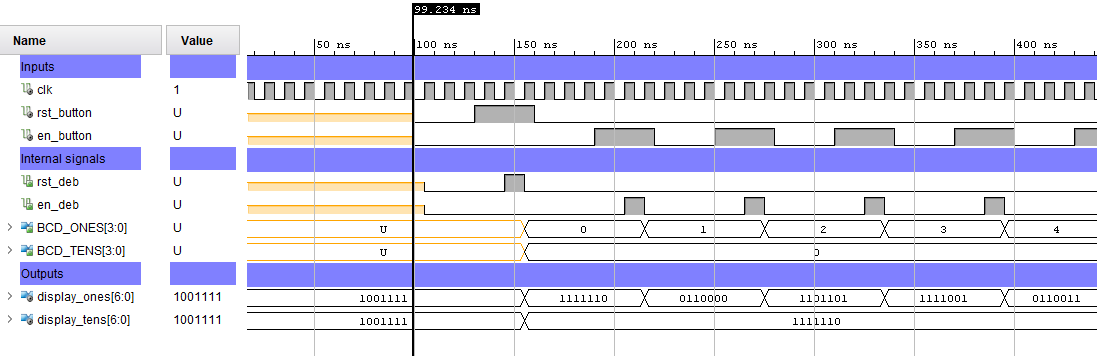
\includegraphics[width=0.9 \textwidth]{timing_diagram_beg.png}}
    \caption{Start of timing diagram}
    \label{fig:Start of Timing Diagram}
\end{figure}

The timing diagram in \autoref{fig:Transition from 09 to 10} shows the transition from 09 to 10 (from ones to tens). This proves that the logic that controls the enable of the tens counter works correctly.

\begin{figure}[ht]
    \centering
    \fbox{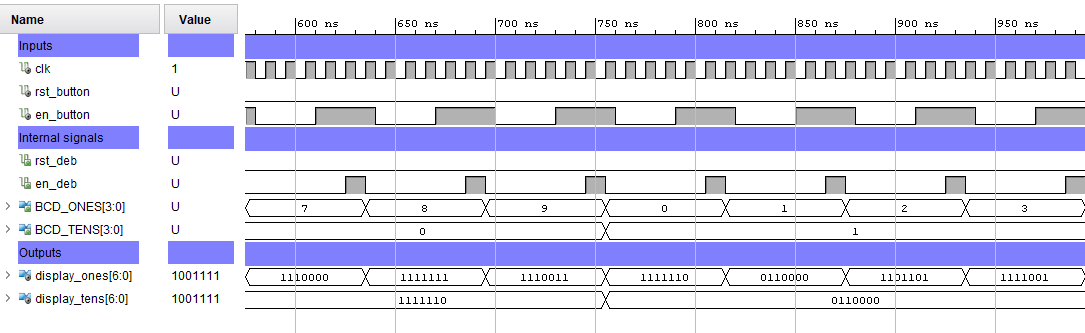
\includegraphics[width=0.9 \textwidth]{timing_diagram_mid.png}}
    \caption{Transition from 09 to 10}
    \label{fig:Transition from 09 to 10}
\end{figure}
\newpage

The timing diagram in \autoref{fig:Transition from 99 to 00} illustrates a successful transition from 99 to 00 (the overflow).

\begin{figure}[ht]
    \centering
    \fbox{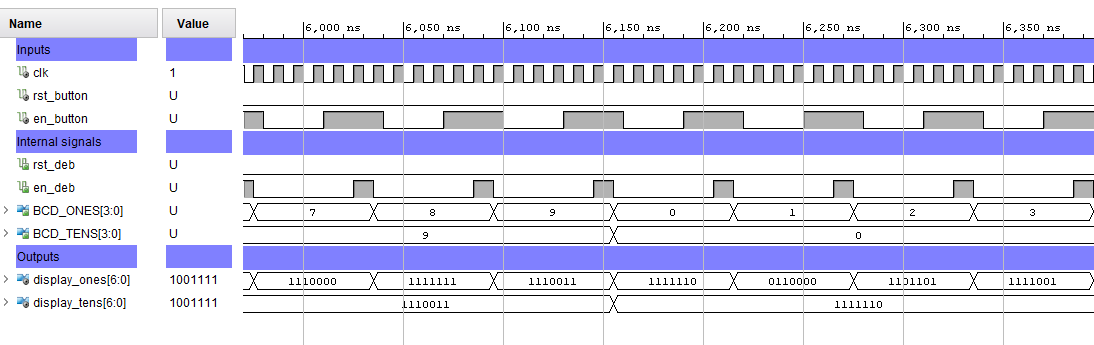
\includegraphics[width=0.9 \textwidth]{timing_diagram_end.png}}
    \caption{Transition from 99 to 00}
    \label{fig:Transition from 99 to 00}
\end{figure}


The timing diagram in \autoref{fig:Reset Procedure} shows that the reset procedure operates successfully since the values in both counters are set to zero.
\begin{figure}[ht]
    \centering
    \fbox{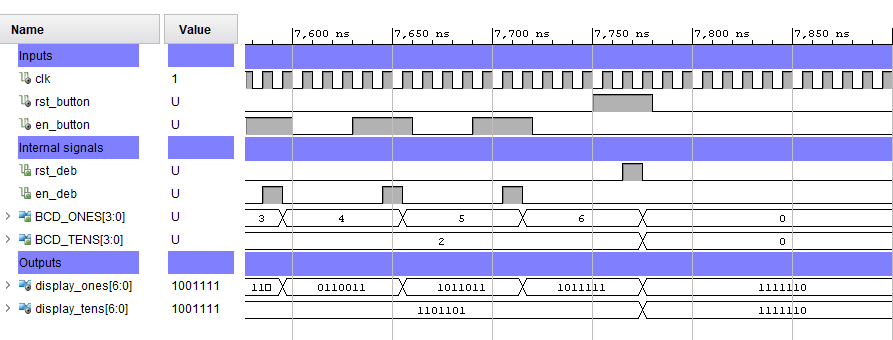
\includegraphics[width=0.9 \textwidth]{timing_diagram_rst.png}}
    \caption{Reset procedure}
    \label{fig:Reset Procedure}
\end{figure}
\newpage

\subsection{RTL Statistics}

In the RTL Hierarchical Component Statistics it can be seen that in the DEBOUNCE module there are three 1-bit registers (or D-FFs) as expected. The bcd\_counter consists of a one 4-bit register with an incremental feedback, which explains the inclusion of the Adder. It also has a clear statement to clear the counter when the output reaches 9. That explains why a multiplexer is included.

It is odd that there is no information regarding the components inside the decoder, which consists of a ROM memory and 9 multiplexers (it can be seen from the schematic displayed in \autoref{fig:Decoder Schematic}).

When it comes to the RTL Component Statistics it just shows the overall number of components used by the implementation of the controller.

\begin{minted}{text}
---------------------------------------------------------------------------------
Start RTL Component Statistics 
---------------------------------------------------------------------------------
Detailed RTL Component Info : 
+---Adders : 
	   2 Input      4 Bit       Adders := 2     
+---Registers : 
	                4 Bit    Registers := 2     
	                1 Bit    Registers := 6     
+---Muxes : 
	   2 Input      4 Bit        Muxes := 2     
---------------------------------------------------------------------------------
Finished RTL Component Statistics 
---------------------------------------------------------------------------------
---------------------------------------------------------------------------------
Start RTL Hierarchical Component Statistics 
---------------------------------------------------------------------------------
Hierarchical RTL Component report 
Module DEBOUNCE 
Detailed RTL Component Info : 
+---Registers : 
	                1 Bit    Registers := 3     
Module bcd_counter 
Detailed RTL Component Info : 
+---Adders : 
	   2 Input      4 Bit       Adders := 1     
+---Registers : 
	                4 Bit    Registers := 1     
+---Muxes : 
	   2 Input      4 Bit        Muxes := 1     
---------------------------------------------------------------------------------
Finished RTL Hierarchical Component Statistics
---------------------------------------------------------------------------------
\end{minted}
\newpage

\subsection{Schematic}

On the schematic in \autoref{fig:Controller Schematic} it can be seen that it is a top level schematic. In other words, all of the separate vhdl files that were included in the controller.vhd (DEBOUNCE.vhd, COUNT.vhd and DECODER.vhd) are shown as their own components.

\begin{figure}[ht]
    \centering
    \fbox{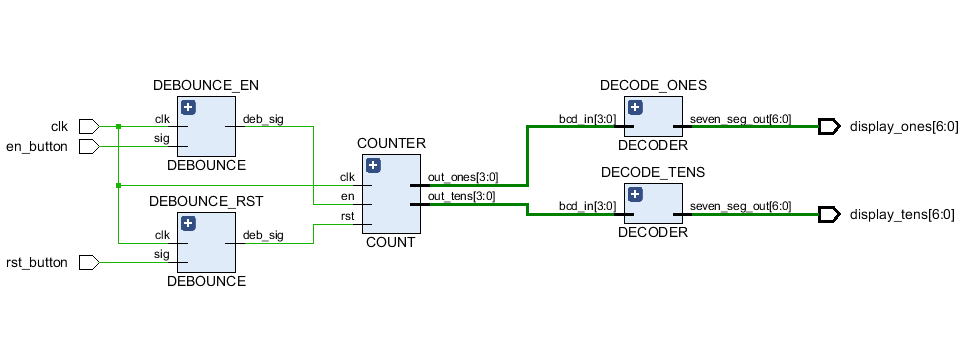
\includegraphics[width=0.9 \textwidth]{lab_2_B_schematic.png}}
    \caption{Controller schematic}
    \label{fig:Controller Schematic}
\end{figure}

The schematic in \autoref{fig:Debounce Schematic} exhibits the hardware implementation of the debounce circuit (DEBOUNCE.vhd). As was mentioned in the RTL statistics in Section 3.7, the implementation uses three separate D-registers, also known as D-type flipflops, and an output word which collects the data of the outputs of those registers and produces the result of the debouncer.
This is to be expected, because there were 3 separate internal STD\_LOGIC\_VECTOR lines in the VHDL file regarding that schematic.

\begin{figure}[ht]
    \centering
    \fbox{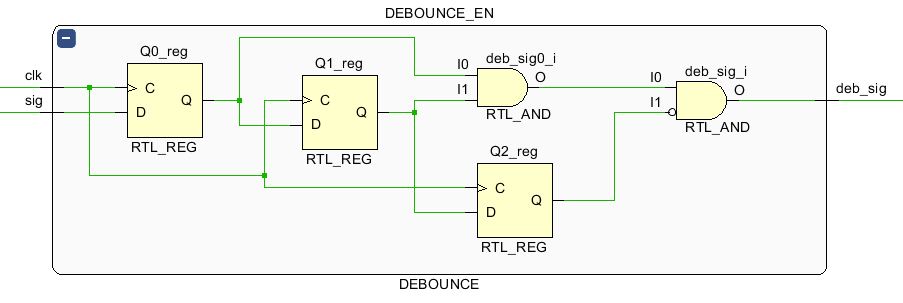
\includegraphics[width=0.9 \textwidth]{debounce_sch.png}}
    \caption{Debounce schematic}
    \label{fig:Debounce Schematic}
\end{figure}

\newpage

The schematic in \autoref{fig:Counter Schematic} is again a top level schematic involving two components which are BCD counters (bcd\_counter.vhd) connected with a logic word that transfers the counting from ones to tens.

\begin{figure}[ht]
    \centering
    \fbox{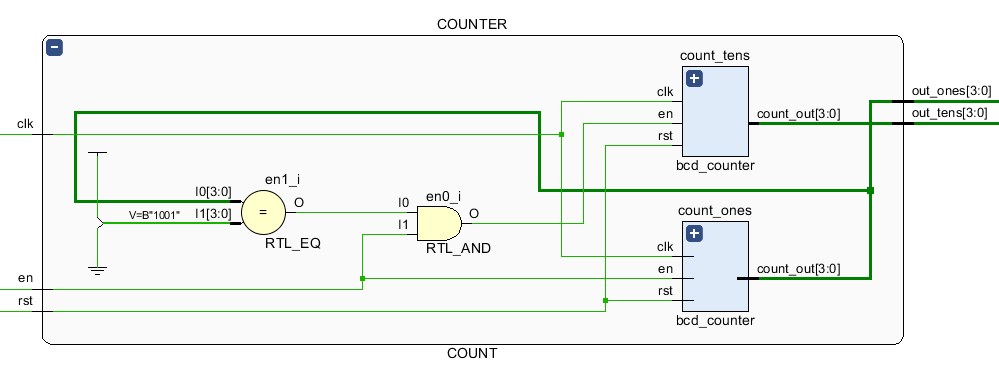
\includegraphics[width=0.9 \textwidth]{count_sch.png}}
    \caption{Counter schematic}
    \label{fig:Counter Schematic}
\end{figure}

The schematic in \autoref{fig:BCD Counter Schematic} seems unusual. One would expect to see a counter element (implemented as 4 T-FFs connected together) and an AND gate getting as input the LSB and the MSB of the output and producing the reset signal.
Perhaps the reason it was implemented in this fashion is that a register that relies on a clock and a multiplexer and an adder that are asynchronous doesn't require any clock division at all. 

Regarding the VHDL code that produced the schematic, it is almost a direct interpretation. In the code there is an UNSIGNED 4-bit bus which is interpreted as a register with synchronous reset and an enable procedure. 

The incrementation of the value is interpreted as a feedback with an adder circuit. Which is directly:
\begin{minted}{VHDL}
    count_internal <= ( count_internal + 1 );
\end{minted}
And the if..else... statement is interpreted as a multiplexer.

\begin{figure}[ht]
    \centering
    \fbox{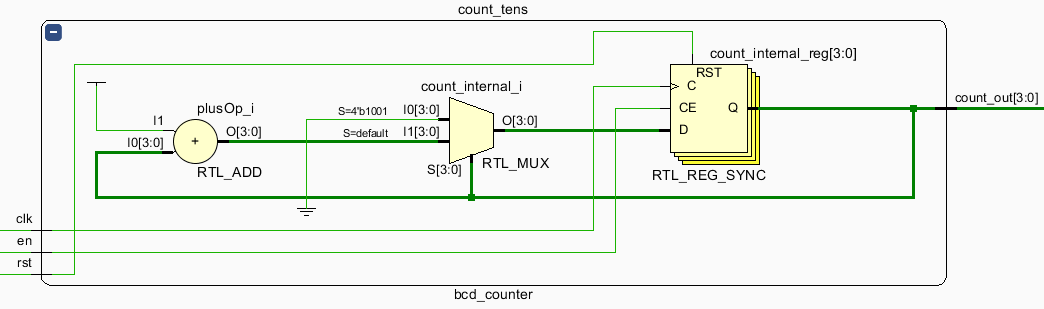
\includegraphics[width=0.9 \textwidth]{BCD_counter_sch.png}}
    \caption{BCD counter schematic}
    \label{fig:BCD Counter Schematic}
\end{figure}
\newpage

The schematic of the Decoder in \autoref{fig:Decoder Schematic} consists of one ROM memory followed by nine multiplexers (seven\_seg\_out\_i\_[0-8]). All of those multiplexers are reacting to a specific input combination (8-0) or passes to the next one. It is perplexing, however, that the combination for the value nine is missing. It may be stored in the ROM memory, but there does not seem to be a way to see what information is stored in this memory.

The implementation using many multiplexers with a default value appears as a direct interpretation of the "... when ... else ..." statement in vhdl syntax.

\begin{figure}[ht]
    \centering
    \fbox{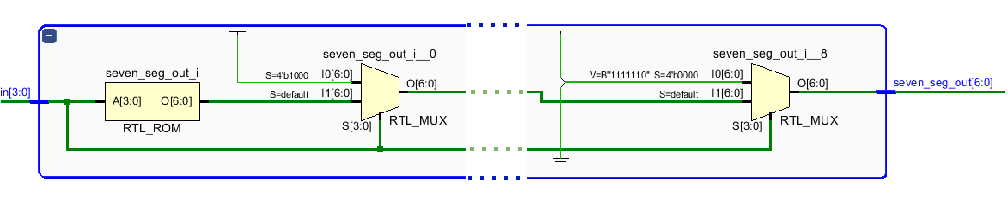
\includegraphics[width=0.9 \textwidth]{decoder_schematic.pdf}}
    \caption{Decoder schematic}
    \label{fig:Decoder Schematic}
\end{figure}
\newpage

\section{Conclusion}
Both of the prescribed tasks were successfully implemented and tested. This lab clearly helped one understand sequential logic and also showed a real life use case of VHDL designs. It also revealed some easy to miss details when implementing digital systems and challenged one to think about the problems in an applicable manner.
\newpage
\section{Appendix}
\subsection{Debounce Implementation \texttt{(DEBOUNCE.vhd)}}
\begin{minted}{vhdl}
library IEEE;
use IEEE.STD_LOGIC_1164.ALL;

-- Implementation of a simple debounce circuit, to be used in a simulation
-- environment. It is not particularly useful in synthesized circuits, 
-- because it requires a steady signal for two clock cycles, which with 
-- 100MHz the clock is 0.02µs. If the input is continuously held at a logic
-- high, the output would be held high for just one clock cycle

entity DEBOUNCE is
    Port ( clk : in STD_LOGIC;        -- Clock signal
           sig : in STD_LOGIC;        -- Input signal
           deb_sig : out STD_LOGIC);  -- Output signal (debounced)
end DEBOUNCE;

architecture Behavioral of DEBOUNCE is

-- Internal signals that hold values in between clock cycles.
signal Q0, Q1, Q2 : STD_LOGIC;

begin

 -- On the rising edge of the clock, the input signal is bit shifted 
 -- to the right along the internal FFs (Q0, Q1, Q2)
 
process (clk) is
begin  
    if (rising_edge(clk)) then
        Q0 <= sig;
        Q1 <= Q0;
        Q2 <= Q1;
    end if;
end process;

-- The output signal gets a logic high when the value of the internal FFs 
-- is 110. The logic high in the first two D-FFs implements the edge 
-- detection. The value '0' in the third FF implements the edge detection

deb_sig <= Q0 and Q1 and (not Q2);
end Behavioral;
\end{minted}
\newpage

\end{document}  